
\chapter{Modelando a Credibilidade com Programação Genética}
\label{cap::programacao_genetica}

No Capítulo~\ref{cap::metodo},
além de mostrarmos os algoritmos de classificação \textit{Naïve Bayes} e \textsc{KNN}, vimos como podemos incorporar a credibilidade aos mesmos.
Discutimos também que existem várias métricas que podem ser utilizadas para mensurar a credibilidade de um exemplo,
embora não detalhamos essas métricas.

Nessa dissertação, modelamos a credibilidade em duas abordagens diferentes, uma levando em consideração os atributos dos exemplos e outra utilizando os seus relacionamentos.
Em ambas somos capazes de gerar uma grande gama de métricas que conseguem capturar a relação entre os exemplos e uma determinada classe, medindo a credibilidade que os exemplos de treino têm para cada classe.
Entretanto, necessitamos de uma forma de selecionar e combinar essas métricas de uma maneira robusta. Para solucionar esse problema, recorremos ao uso de Programação Genética (\textsc{PG}) (\cite{Koza92}).

Segundo a Teoria da Evolução de Darwin, indivíduos mais adaptados ao ambiente em que se encontram têm uma chance maior de sobreviverem e se reproduzirem, passando seu material genético às gerações posteriores. Baseado nessa teoria, o método de Programação Genética é adequado para evoluir uma função de credibilidade, pois possui mecanismos de busca que o torna capaz de explorar bem o imenso espaço de soluções formado pelo grande número de métricas disponíveis (\cite{Fogel00}). Além disso, \textsc{PG} é flexível o bastante para ser capaz de representar as funções que desejamos, sendo também tolerante a ruído.
%Programação Genética é um método baseado na Teoria da Evolução de Darwin que define que indivíduos mais adaptados ao ambiente em que se encontram têm uma maior chance de sobreviverem e se reproduzirem, passando seu material genético às gerações posteriores. PG é um método adequado para evoluir uma função de credibilidade, pois consegue explorar bem o imenso espaço de soluções formado pelo grande número de métricas disponíveis e é flexível o bastante para podermos representar as funções que desejamos.

Para entendermos melhor como é o funcionamento de um \textsc{PG}, utilizamos a Figura~\ref{fig::gpwf}. Ela ilustra o comportamento do arcabouço de Programação Genética usado pelo pacote \textit{gpc++} (\cite{gpcpp}), usado em todos os experimentos dessa dissertação. Mesmo se tratando de um arcabouço com várias especificidades, ele pode ser facilmente adaptado para considerar as especifidades do problema aqui apresentado.
Como podemos ver, o primeiro passo de qualquer \textsc{PG} é definir um conjunto de funções e terminais para serem usados pelo \textsc{PG}.
É a partir desse conjunto de elementos que criamos nossos indivíduos.
Esses, por sua vez, são soluções candidatas para o problema que abordamos.
%(no caso, um indivíduo é uma possível função de credibilidade).

Um conjunto de indivíduos é chamado de população e, como mostrado pelo segundo retângulo no diagrama da Figura~\ref{fig::gpwf}, a população inicial é criada aleatoriamente, utilizando o método \textit{Ramped-Half-and-half}, que garante que metade dos indivíduos sejam representados por árvores de tamanhos variados e a outra metade por árvores completas.
Cada indivíduo da população é então avaliado por uma função de \textit{fitness}, que calcula a habilidade do mesmo em resolver o problema apresentado, ou seja, o quão bom aquele indivíduo é.

\begin{figure}[t]
\centering
%\includegraphics[width=1.0\textwidth]{figures/gpwf.png}
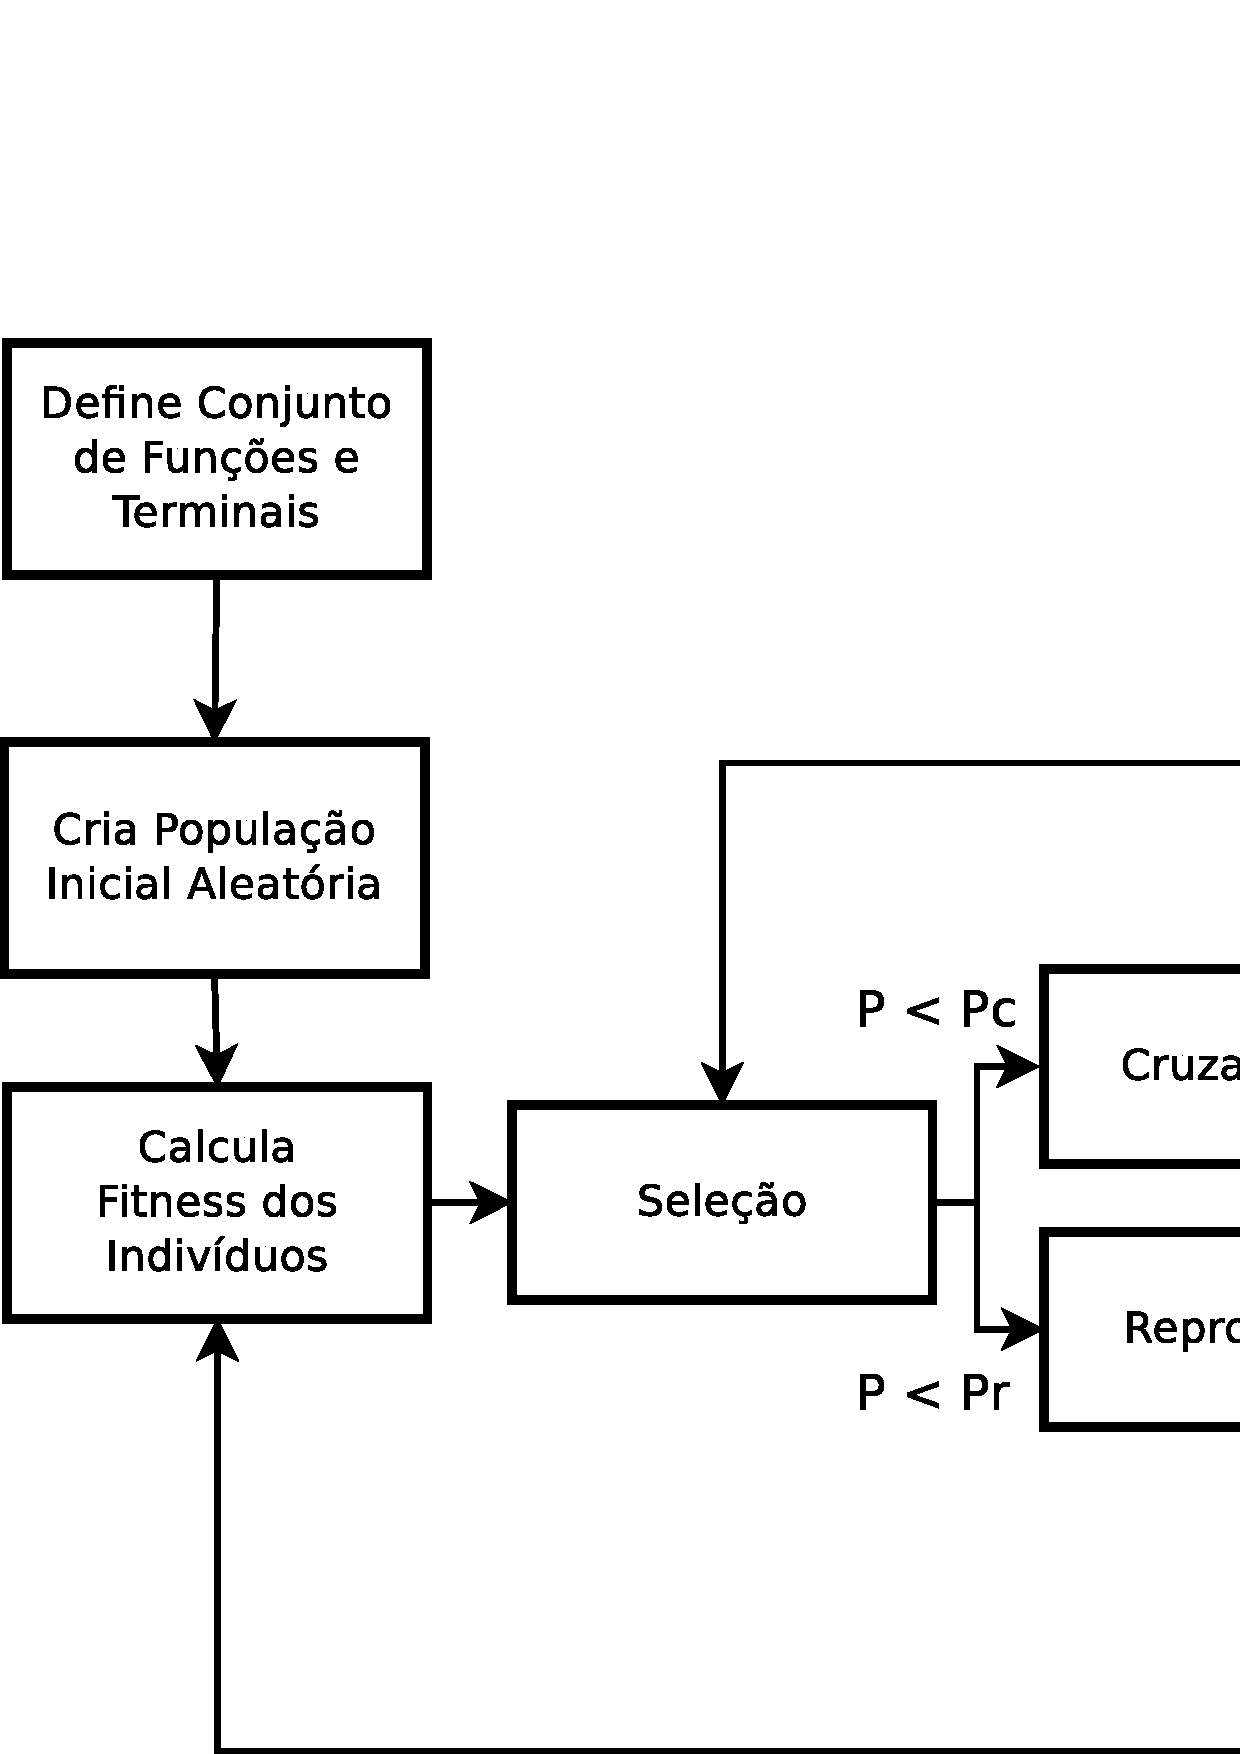
\includegraphics[width=1.1\textwidth]{figures/gpwf_new.png}
\caption{Fluxograma de um algoritmo de Programação Genética}
\label{fig::gpwf}
\end{figure}

Após avaliarmos a \textit{fitness} dos indivíduos, os melhores são selecionados e submetidos às operações genéticas de cruzamento, reprodução e mutação, com probabilidade $P_c$, $P_r$ e $P_m$, respectivamente, definidas pelo usuário.
Uma forma muito usada de selecionar os indivíduos é através de torneios, nos quais tomamos aleatoriamente um número pré-definido de indivíduos da população e selecionamos aquele com maior valor da função de \textit{fitness}. Existem diversas outras variações do método de seleção (\cite{Koza92}), sendo que o importante é utilizar a função \textit{fitness} dos indivíduos de forma a criamos uma próxima geração mais bem preparada para resolução do problema.

Depois de serem selecionados, os indivíduos podem passar por reprodução ou cruzamento, com probabilidades $P_r$ e $P_c$, respectivamente.
A operação genética de reprodução simplesmente transfere o indivíduo para próxima geração, enquanto o cruzamento exige a participação de dois indivíduos que são combinados a fim de obtermos
uma prole mais adaptada na próxima geração.
Após esse processo, o indivíduo resultante da reprodução ou cruzamento pode ser submetido à mutação com uma probabilidade $P_m$.
Em geral, a mutação é uma pequena alteração em alguma parte específica do indivíduo, mudando uma função interna ou um terminal.
Variações nas quais a operação de mutação ocorre em paralelo a de reprodução ou cruzamento também são comuns na literatura.

Esse processo de criação de indivíduos é repetido até atingirmos o tamanho limite para a população. Após chegarmos a esse limite, uma nova geração é iniciada.
O processo então é repetido, geração a geração, até que um limite de gerações seja alcançado.
Outras condições de parada do \textsc{PG} seriam chegar a uma variação arbitrariamente pequena de melhoria de uma geração para outra ou conseguir algum indivíduo com um valor de \textit{fitness} pré-definido. Por fim, o \textsc{PG} retorna o melhor indivíduo evoluído.

%Depois de serem selecionados, os indivíduos podem sofrer alguma alteração genética através das operações de mutação e cruzamento ou podem ser transferidos diretamente para a próxima geração, através da reprodução.
%a operação de mutação, uma parte do indivíduo selecionado é aleatoriamente alterada, buscando obter uma melhoria da \textit{fitness} na próxima geração.
%or sua vez, a operação de cruzamento exige a participação de dois indivíduos que são combinados a fim de obtermos uma prole mais adaptada na próxima geração.
%o modo como está mostrado na Figura~\ref{fig::gpwf}, somente uma dessas três operações é realizada em cada indivíduo selecionado, entretanto é comum também implementações em que é aplicada a probabilidade de mutação para todos os indivíduos, logo após uma nova prole ser gerada pelo cruzamento ou reprodução.

Repare que todo o processo exposto na Figura~\ref{fig::gpwf} é \textit{independente} da aplicação na qual o \textsc{PG} é utilizado.
Entretanto, três importantes componentes devem ser instanciados dependendo do contexto no qual trabalhamos. Eles são:
\begin{enumerate}
\item A representação dos indivíduos, que incluí as funções do \textsc{PG} e terminais relevantes à aplicação, e são abordados na Seção~\ref{subsec::individuos},
\item Os operadores genéticos, descritos na Seção~\ref{subsec::operadoresgeneticos},
\item A função de \textit{fitness} detalhada na Seção~\ref{subsec::fitness}.
\end{enumerate}
%>> RETIRAR?! Além disso, pelo fato de termos uma vasta gama de terminais e queremos explicar um por um deles, separamos as Seções~\ref{sec::pg_cred_baseada_conteudo} e \ref{sec::pg_cred_baseada_grafos} para explicarmos com detalhes as métricas baseadas em atributos e em relacionamentos, respectivamente.

\section{Indivíduos}
\label{subsec::individuos}

Uma parte essencial da construção de um \textsc{PG} é definir a representação dos indivíduos que compõem a população.
Para isso, temos que focar em três aspectos primordiais: o que um indivíduo representa, quais são suas funções e quais são os seus terminais.
%Independente de quais são as funções internas e terminais escolhidos, o propósito de um indivíduo no \textsc{PG} modelado é representar uma função de credibilidade que, a não ser que seja dito o contrário, relaciona um exemplo de teste, seja por seus atributos ou relacionamentos, a uma classe, retornando um valor real.

A representação de um indivíduo é dependente das características do problema que estamos lidando.
Portanto, o primeiro passo deve ser estudar a base de dados do problema para saber se podemos utilizar a credibilidade de atributos e/ou de relacionamentos e, se usarmos a credibilidade de relacionamentos, quantos e quais relacionamentos podem ser explorados.
Por exemplo, em uma base de dados de documentos, os termos dos documentos seriam usados para criarmos uma função de credibilidade de atributos e os relacionamentos de autoria e/ou citação seriam usados para criarmos funções de credibilidade de relacionamentos. Entretanto, se estivermos tentando resolver um problema em que não existam informações para inferirmos relacionamentos, então usaremos somente os atributos. O caso contrário também é possível.

Como inicialmente discutido no Capítulo~\ref{cap::metodo}, criamos uma função de credibilidade referente a cada dimensão que trabalhamos, ou seja, uma função para os atributos e uma para cada relacionamento utilizado. Dessa forma, um indivíduo é composto por um \textbf{conjunto} de funções de credibilidade que são usadas para melhorarmos os algoritmos de classificação empregados.
As Figuras~\ref{fig::gps1} e~\ref{fig::gps2} mostram cinco exemplos de funções de credibilidade que podem ser geradas pelo \textsc{PG}. As três contidas na primeira figura ilustram funções de credibilidade baseadas em atributos e as demais são baseadas em relacionamentos entre os exemplos\footnote{As cores são usadas apenas para auxiliar na explicação das operações genéticas de mutação e cruzamento na Seção~\ref{subsec::operadoresgeneticos}}.
Exemplificando, se o problema apresentar a possibilidade de explorarmos a credibilidade de atributos e de dois relacionamentos, então um possível indivíduo do \textsc{PG} poderia ser formado por uma das funções de credibilidade mostradas na Figura~\ref{fig::gps1} e das duas funções da Figura~\ref{fig::gps2}, uma para cada relacionamento.

%e~\ref{fig::gps2}
%Nesse trabalho, um indivíduo é modelado para representar funções de credibilidade para os relacionamentos e atributos, como discutido nas Seções~\ref{subsubsec::nbcredatributos} e \ref{subsubsec::nbcredgrafos} para o \textit{Naïve Bayes} e Seções~\ref{subsubsec::knncredatributos} e \ref{subsubsec::knncredgrafos} para o \textsc{KNN}.

Como vemos nas Figuras~\ref{fig::gps1} e \ref{fig::gps2}, as funções de credibilidade apresentam a estrutura de árvore, comuns em trabalhos com \textsc{PG} (\cite{Koza92}).
Árvores, em suma, são estruturas de dados semelhantes aos grafos, porém sem ciclos, ou seja, ao se percorrer as arestas a partir de um determinado vértice, não podemos voltar àquele vértice
%\footnote{Recomendamos para maior entendimento a respeito de árvores, a leitura do Capítulo 2.3 de~\cite{Knuth97}.}
.
%O nome ``árvore'' vem do fato que essa estrutura de dados se assemelhar a uma árvore, encontrada em qualquer jardim, quando vista de cabeça para baixo.
%Mesmo não sendo uma analogia tão boa, essa estrutura de dados é muito comum na área de Ciência da Computação, sendo excelente para a representação de funções, entre outras tarefas.
Pedimos a atenção do leitor para o fato que em qualquer árvore existem dois tipos diferentes de vértices, os internos e os externos.
Os vértices externos recebem o nome especial de folha e em nossas árvores representam as métricas de credibilidade usadas.
Já os vértices internos são operadores usados para interconectar as folhas da árvore. Se observarmos a função 2 na Figura~\ref{fig::gps1}, os vértices internos são o ``+'' e o ``\%'', enquanto os externos são \textsc{AM(x,c)}, \textsc{P(x|c)} e \textsc{IG(x,c)}, métricas usadas para estimar a credibilidade de atributos.

\begin{figure}[!ht]
\centering
%\subfloat[Individuo 1:\newline \hspace*{6mm}$\textsc{GINI}(x)^{\textsc{CC}(x,c)}$]{
\subfloat[Função 1:\newline \hspace*{6mm}$\textsc{GINI}(x)^{\textsc{CC}(x,c)}$]{
    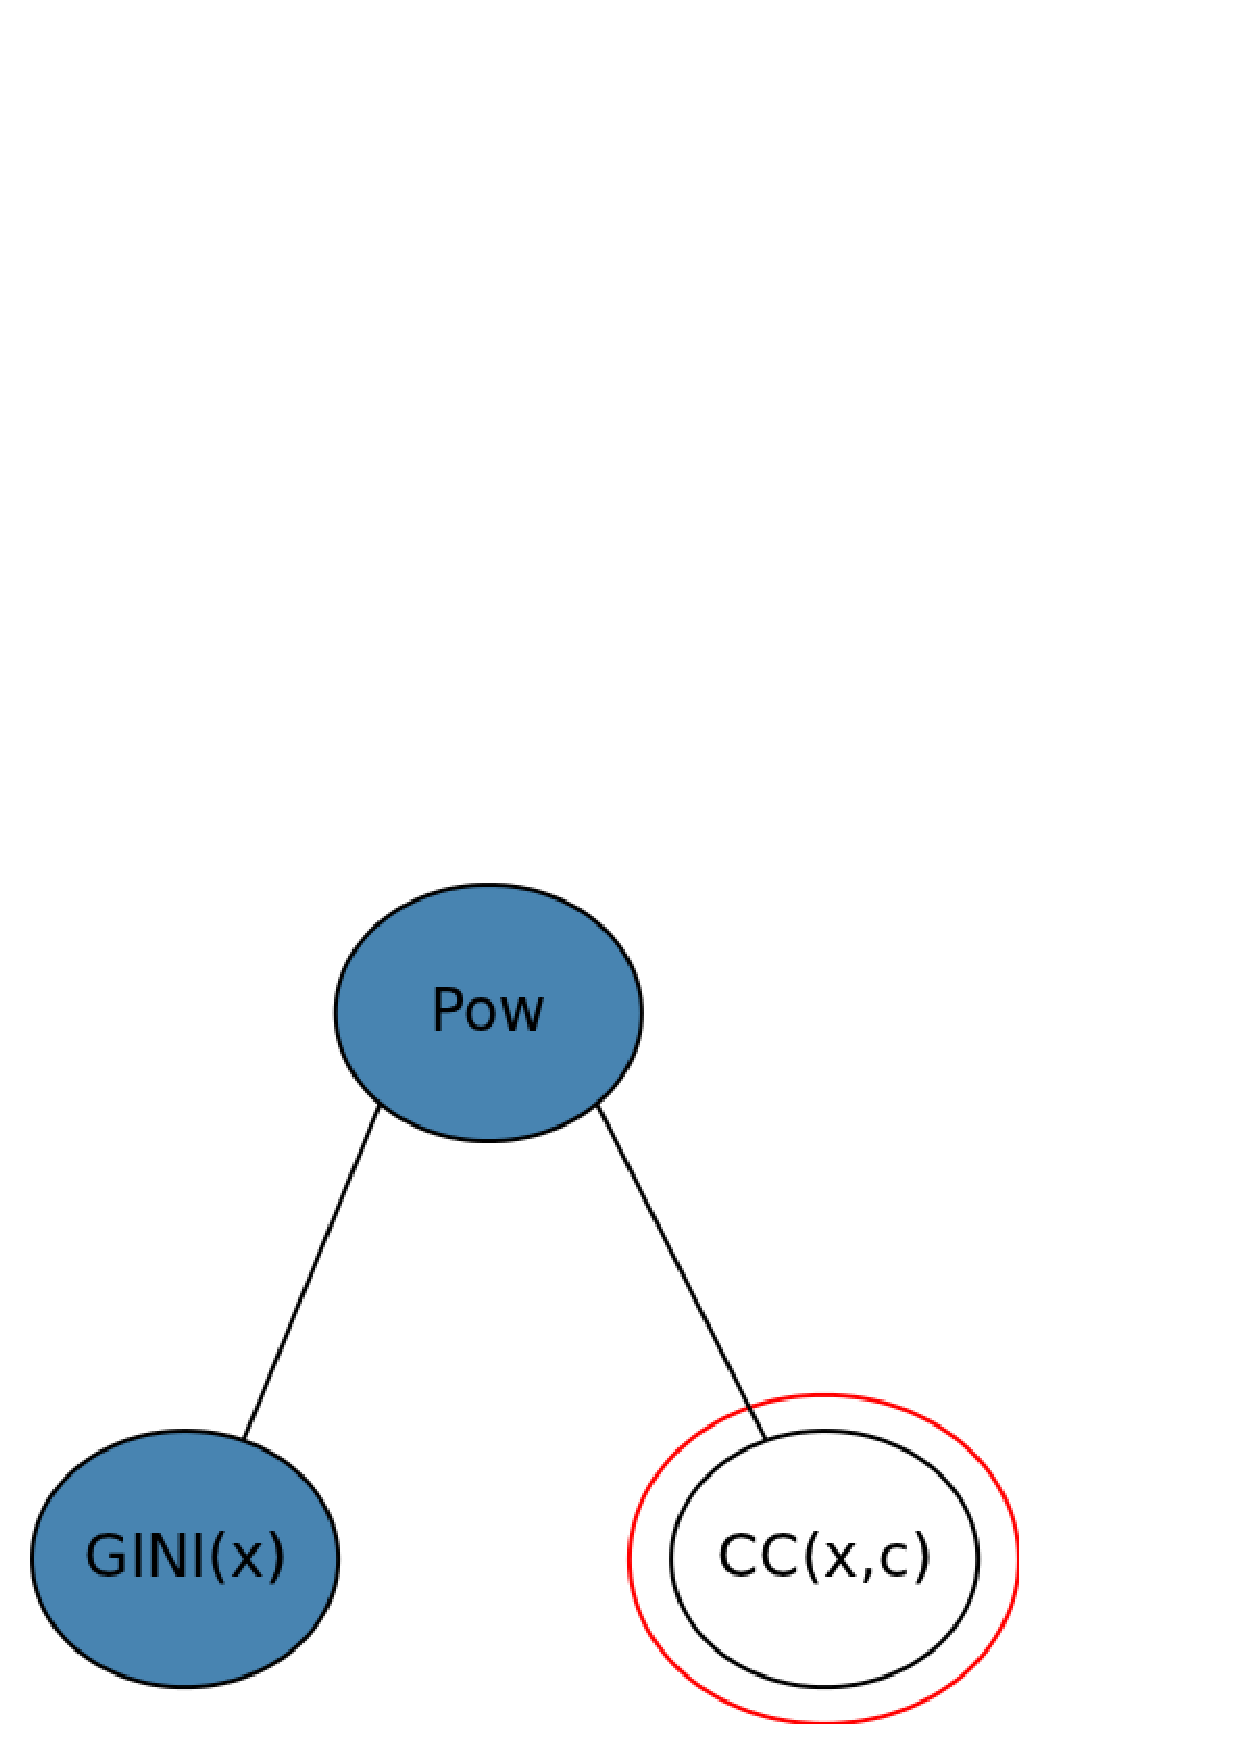
\includegraphics[width=0.25\textwidth]{figures/gp1c.png}
}
\subfloat[Função 2:\newline \hspace*{4mm} $(\textsc{AM}(x,c) + \textsc{P}(x|c)) \% (\textsc{IG}(x,c))$]{
    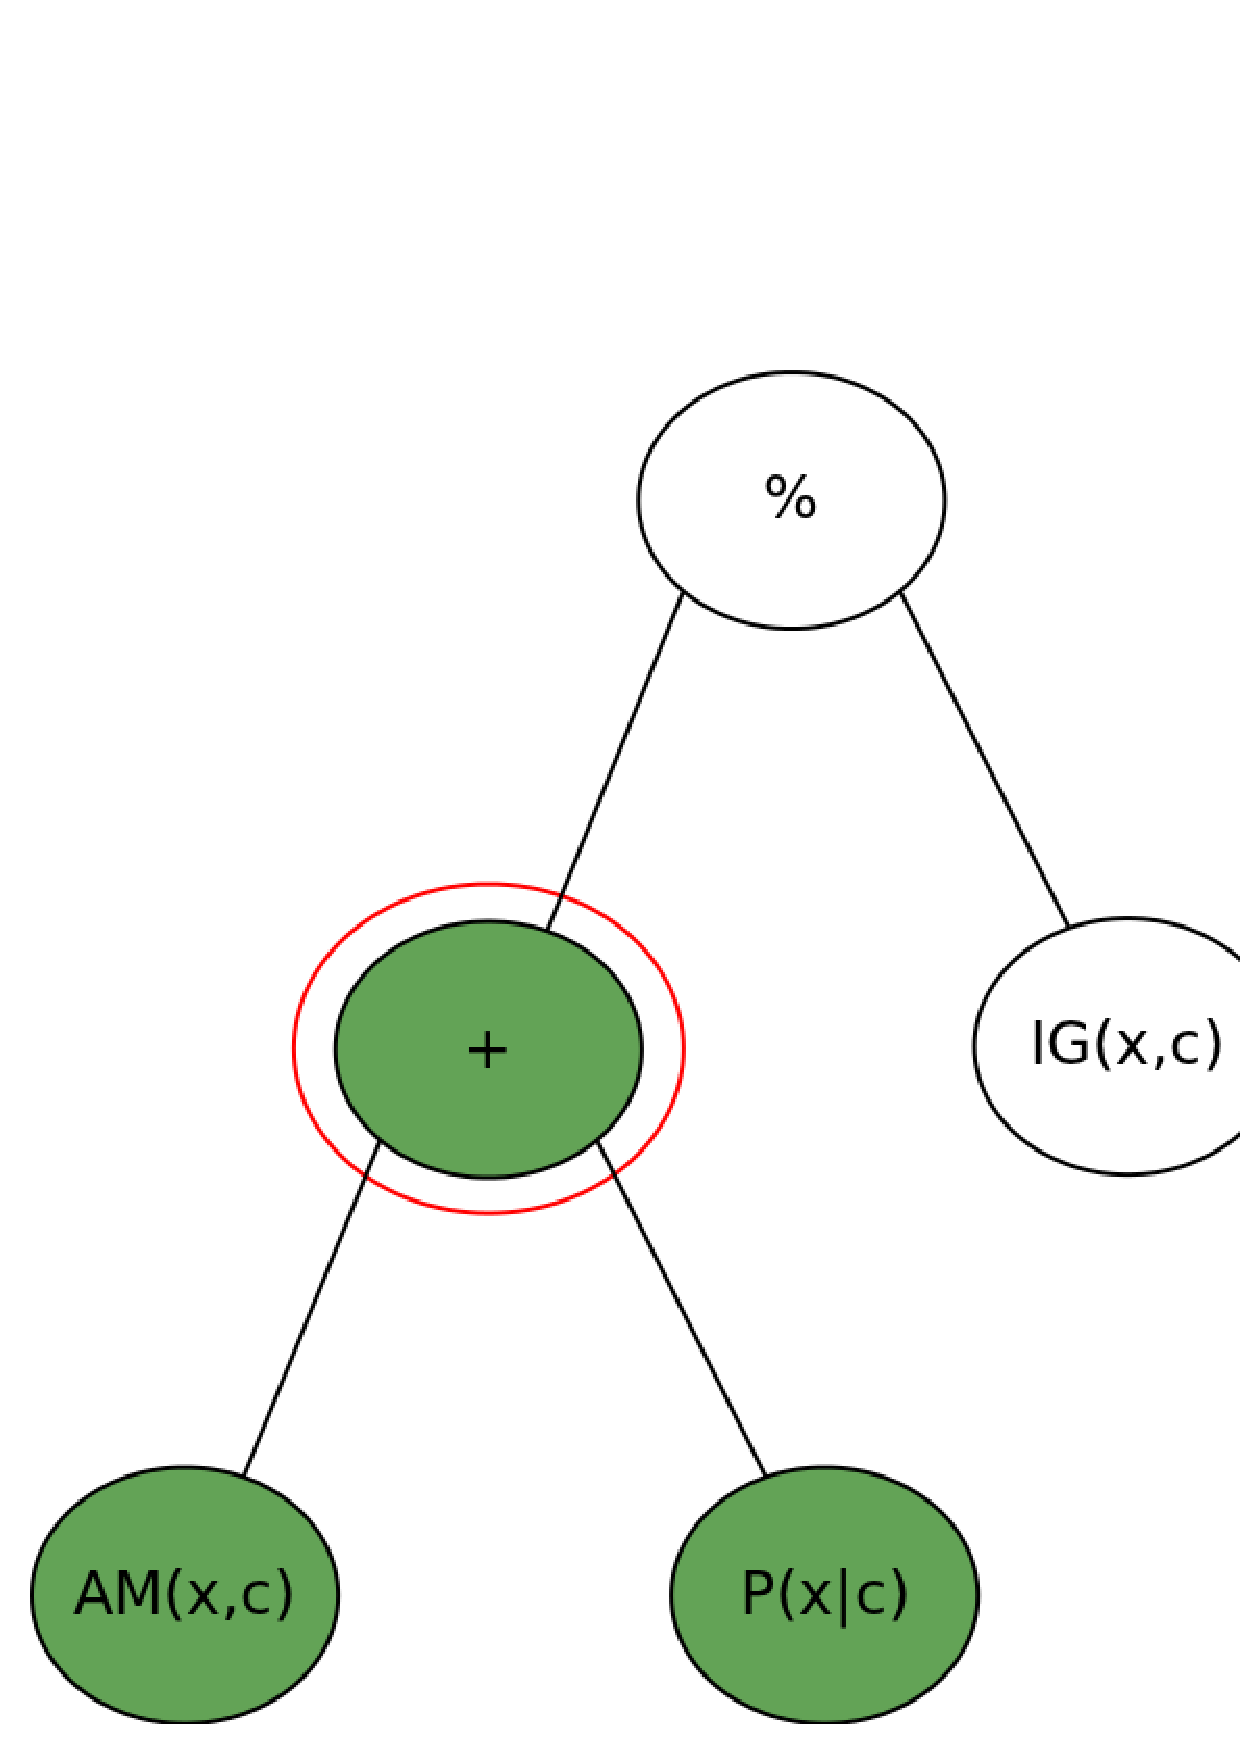
\includegraphics[width=0.33\textwidth]{figures/gp2c.png}
}
\subfloat[Função 3:\newline \hspace*{4mm} $\textsc{GINI}(x)^{(\textsc{AM}(x,c)\ + \ \textsc{P}(x|c))}$]{
    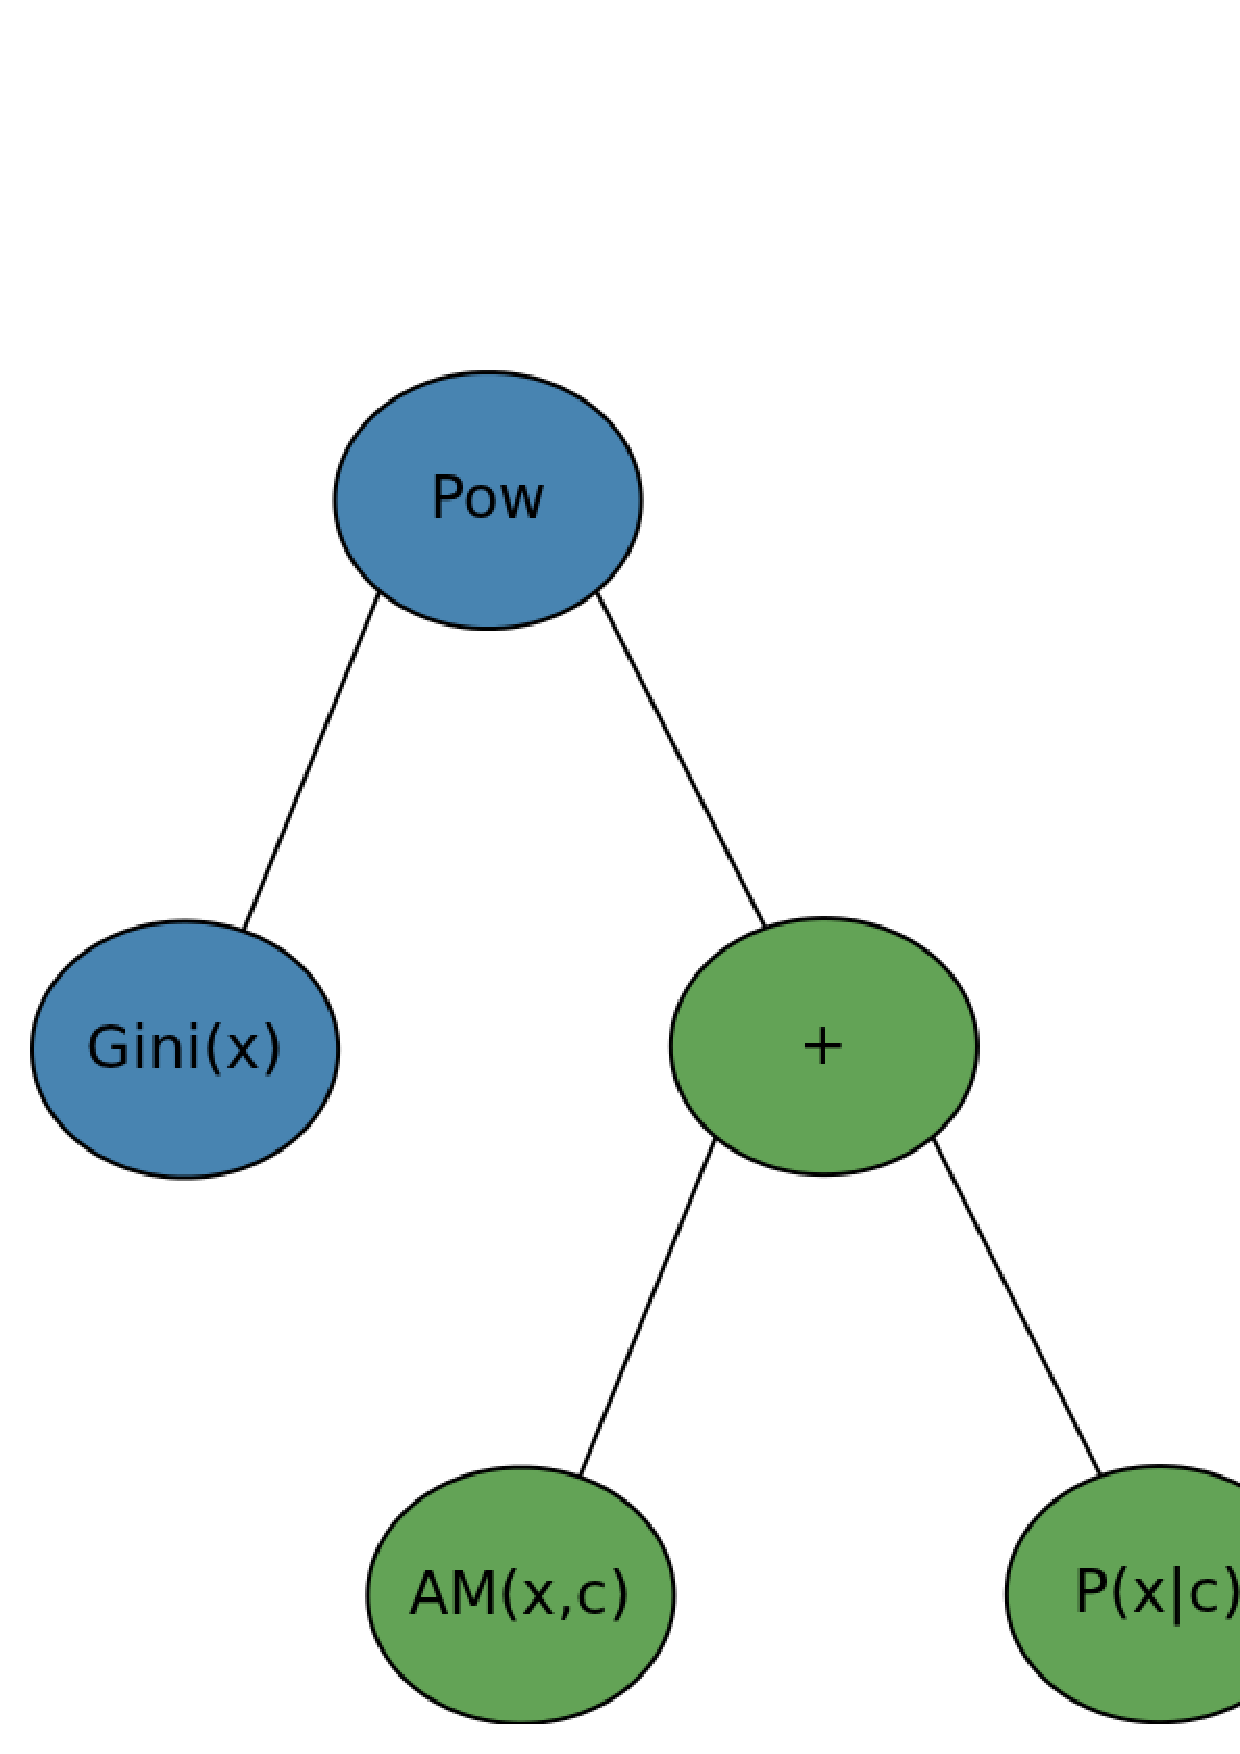
\includegraphics[width=0.33\textwidth]{figures/gp3c.png}
}
\caption{Três possíveis funções de credibilidade de atributos.}
\label{fig::gps1}
\end{figure}


\begin{figure}[!ht]
\centering
\subfloat[Função 1:\newline \hspace*{6mm}$\textsc{Bib}(X,c) - {\textsc{Hub}(x,c)}$]{
%\subfloat[Individuo 1:$\textsc{Bib}(X,c) - {\textsc{Hub}(x,c)}$]{
    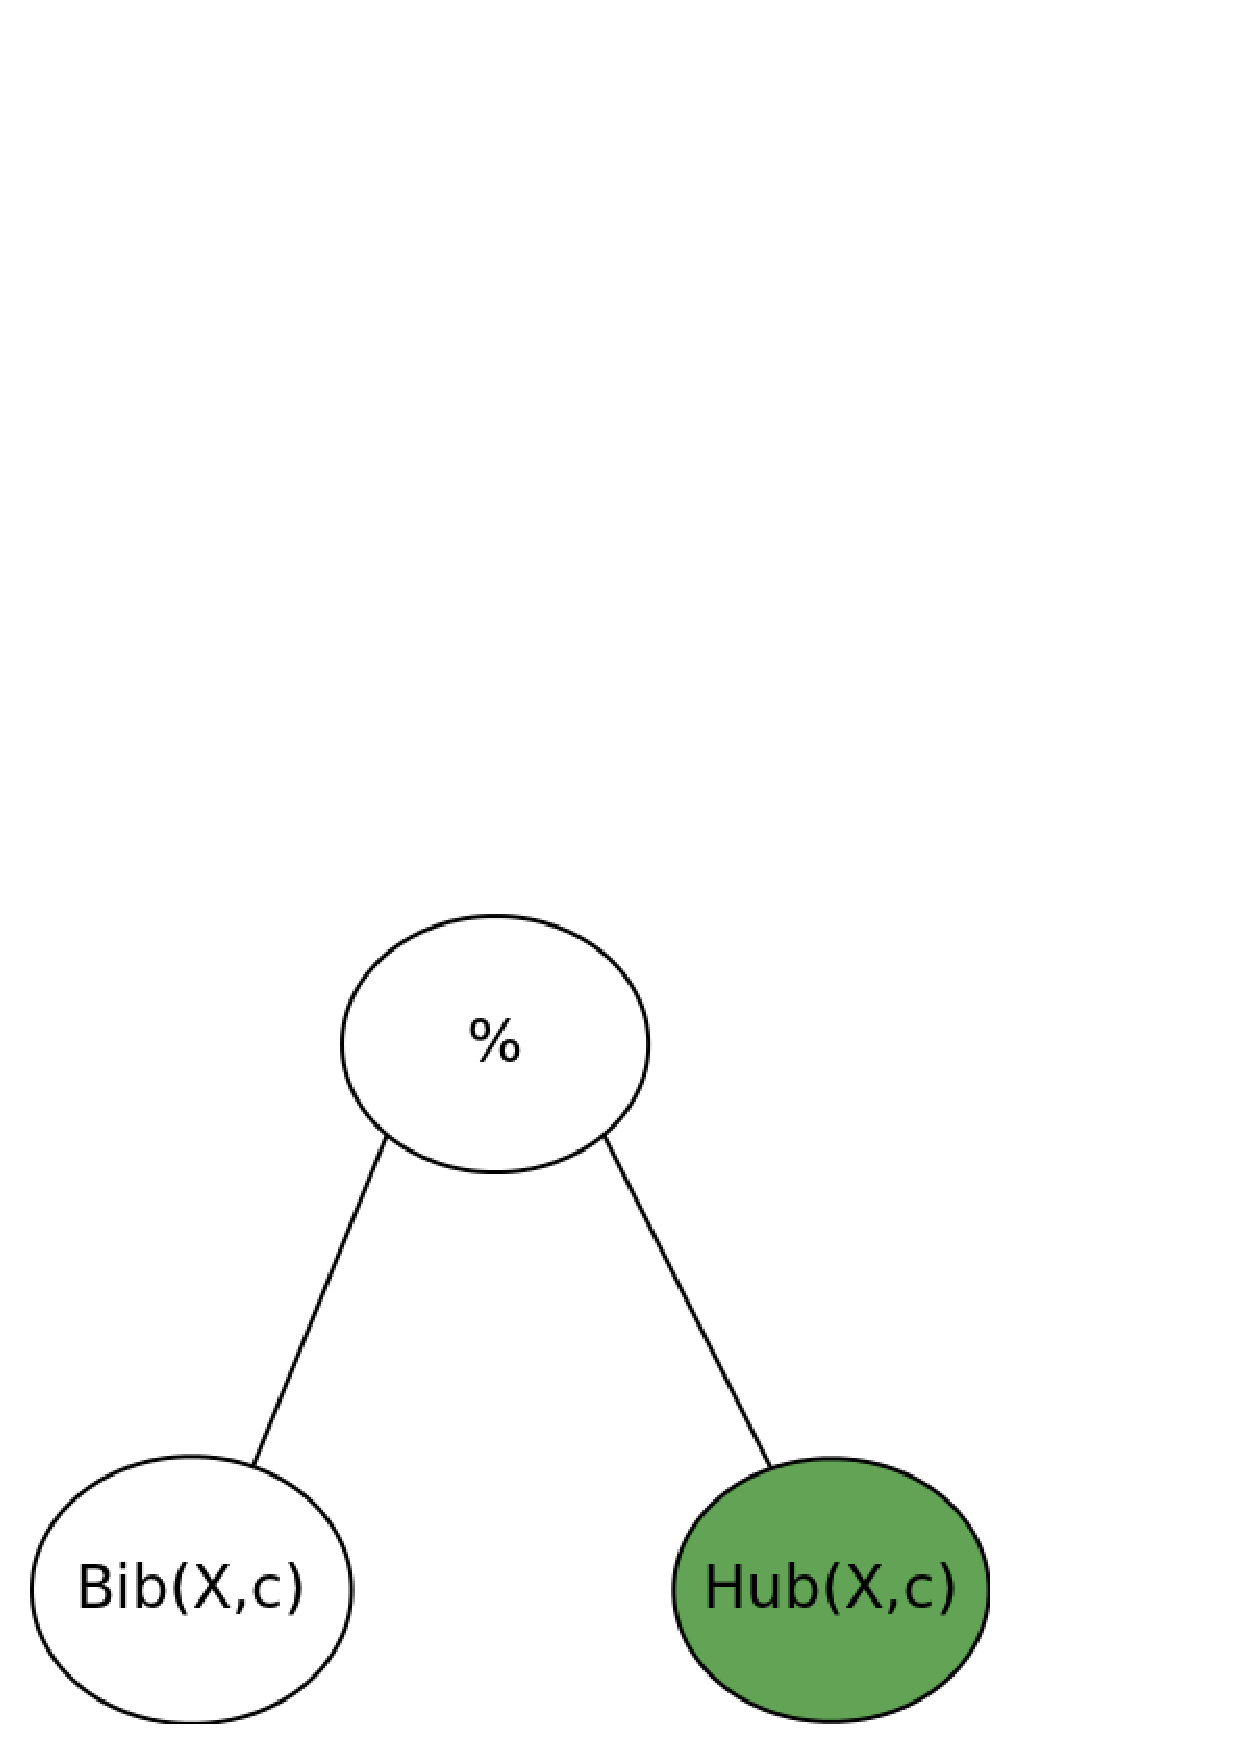
\includegraphics[width=0.30\textwidth]{figures/gp1c_grafos.png}
}
\subfloat[Função 2:\newline \hspace*{5mm} $\textsc{Bib}(X,c) - \textsc{PR}(X,c) $]{
    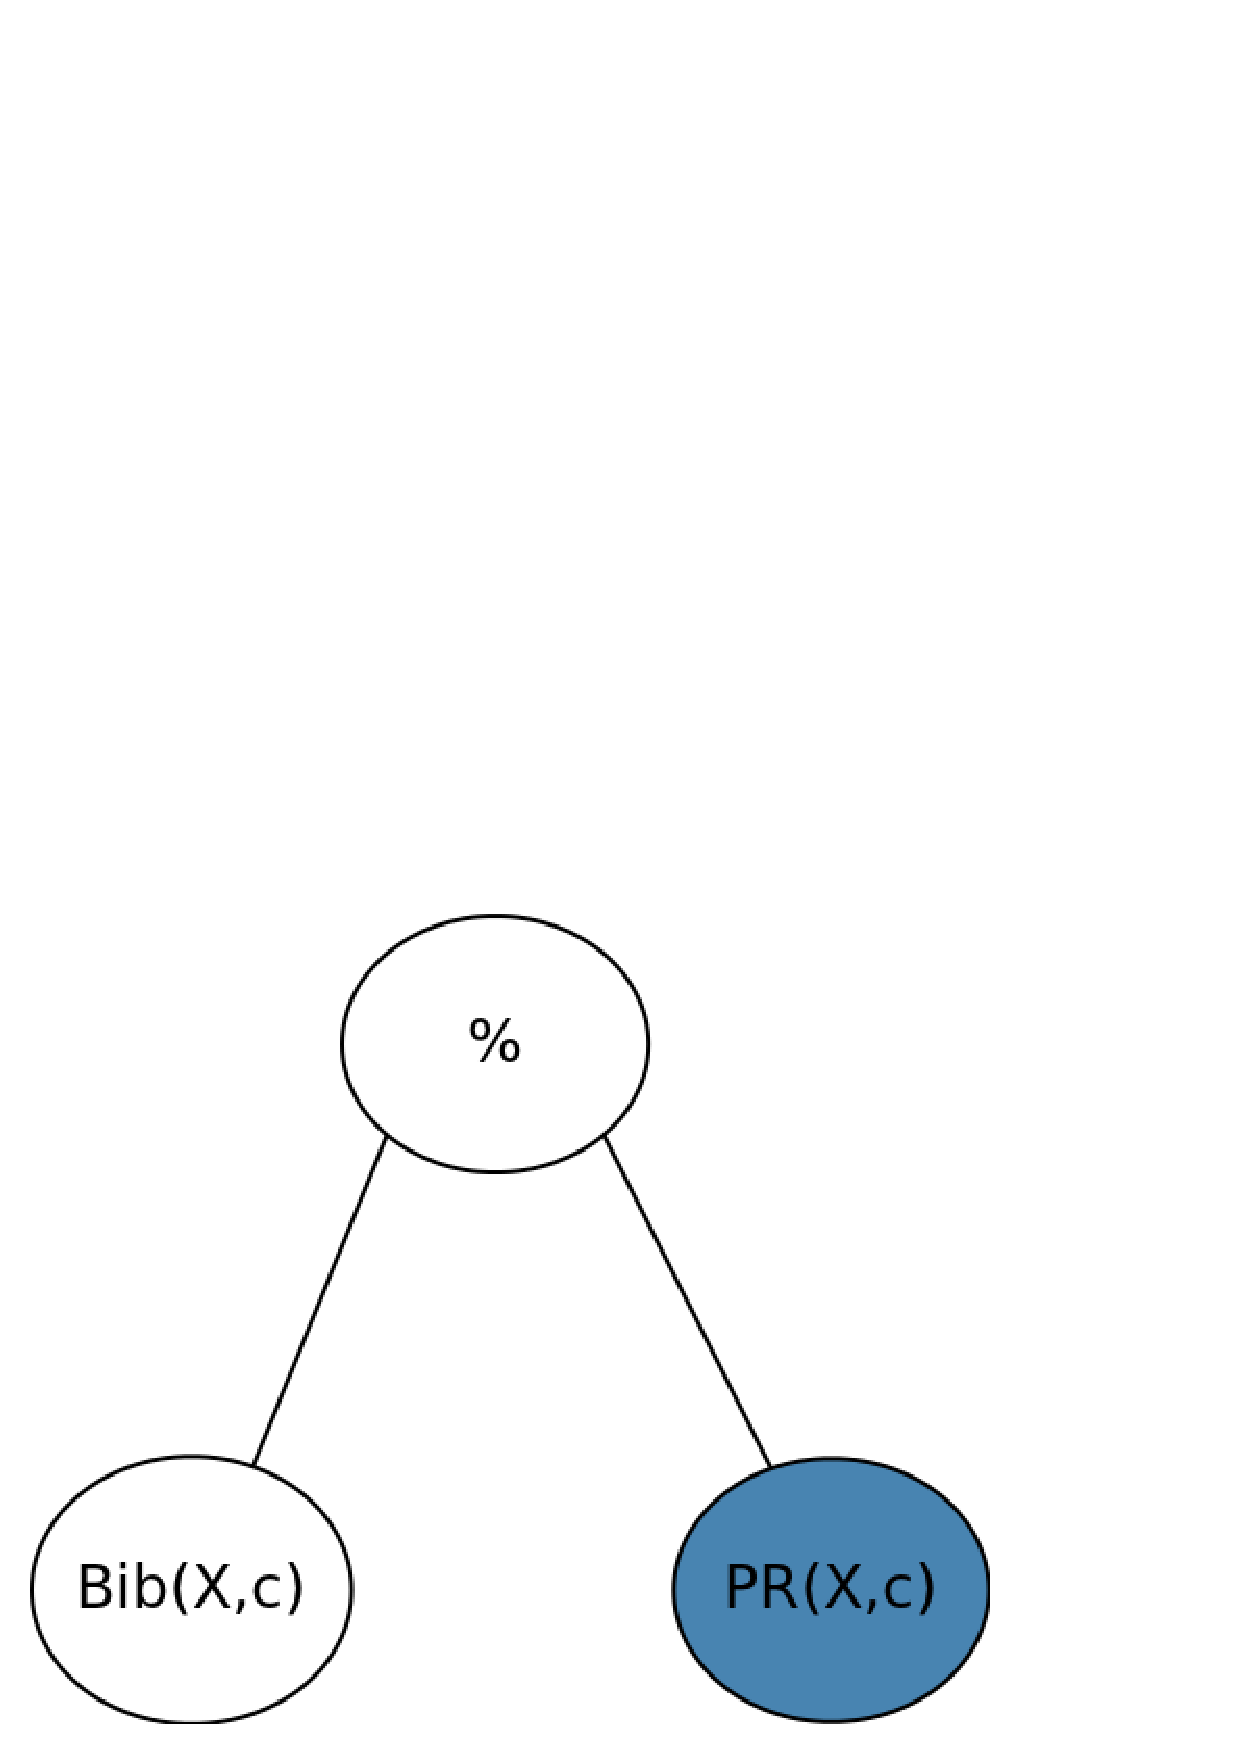
\includegraphics[width=0.30\textwidth]{figures/gp2c_grafos.png}
}
%\caption{Dois possíveis indivíduos gerados para representar uma função de credibilidade para relacionamentos.}
\caption{Duas possíveis funções de credibilidade para relacionamentos.}
\label{fig::gps2}
\end{figure}



%Por questão de espaço e para não tornar esse texto enfadonho, não iremos entrar em detalhes de como podemos ler as funções representadas nas árvores.
%Logo, com exceção das Figuras~\ref{fig::gps1} e \ref{fig::gps2}, optamos por mostrar as funções de credibilidade diretamente em notação matemática.


%Modelamos duas funções de credibilidade diferentes, uma baseada nos atributos dos exemplos e outra baseada nos relacionamentos dos mesmos.
Na Tabela~\ref{table::funcoespg}, mostramos a lista completa de funções do \textsc{PG} usadas.
Como usual para um \textsc{PG} que evolui uma função matemática numérica, as funções \textsc{PG} se consistem de operações matemáticas conhecidas, como a multiplicação, divisão, soma, entre outros. Observe que modificamos as funções de subtração, divisão e logaritmo.
Tanto a divisão por zero, quanto o logaritmo de números negativos não são matematicamente definidos.
Além disso, não queremos ter uma função de credibilidade negativa, e por isso evitamos que a subtração e o logaritmo retornem números negativos.
Portanto, tratamos todos esses casos explicitamente retornando zero.

%Ambas, entretanto, compartilham o mesmo conjunto de funções internas, porém os terminais utilizados são diferentes para cada caso. As funções internas são utilizadas para que haja uma interação entre os terminais.
%Como usual para um \textsc{PG} que evolui uma função matemática numérica, as funções internas do \textsc{PG} consistem de funções matemáticas conhecidas, como a multiplicação, divisão, soma, entre outros que estão mostradas na Tabela
%~\ref{table::funcoespg}.
%Observe que modificamos as funções de subtração, divisão e logaritmo.
%Tanto a divisão por zero, quanto o logaritmo de números negativos não são matematicamente definidos, portanto explicitamente tratamos esses casos retornando zero. Além disso, não queremos ter uma função de credibilidade negativa, portanto evitamos que a subtração e o logaritmo retornem números negativos.

\begin{table}[ht*]
\centering
\caption{Funções do \textsc{PG}, são usadas como vértices internos no \textsc{PG}}
\begin{tabular}{|c||l|}
\toprule
    \textbf{Função Interna} & \textbf{Explicação} \\
\midrule
\hline
    +$(a,b)$           & Soma $a$ com $b$. \tabularnewline \hline
    -$(a,b)$           & Subtrai $b$ de $a$, porém retorna 0 se $b$ for maior que $a$.\tabularnewline \hline
    $\times(a,b)$       & Multiplica $a$ com $b$. \tabularnewline \hline
    \%$(a,b)$          & Divide $a$ por $b$, porém retorna 0 se $b$ for 0. \tabularnewline \hline
    $\text{Pow}(a,b)$  & Eleva $a$ a potência de $b$. \tabularnewline \hline
    $\log(a,b) $       & Logaritmo de $a$ na base $b$, retorna 0 se $a$ ou $b$ forem menores que 1. \tabularnewline
\bottomrule
\end{tabular}
\label{table::funcoespg}
\end{table}

%Pelo fato de termos um grande número de terminais definidos, reservamos as Seções~\ref{sec::pg_cred_baseada_conteudo} e~\ref{sec::pg_cred_baseada_grafos} exclusivamente para descrevermos aqueles relacionados aos atributos e aos relacionamentos, respectivamente.
Pelo fato de termos um grande número de terminais definidos, subdividimos essa seção nas Seções~\ref{sec::pg_cred_baseada_conteudo} e~\ref{sec::pg_cred_baseada_grafos} exclusivamente para descrevermos as métricas relacionadas ao atributos e aos relacionamentos entre os exemplos, respectivamente.

\input{04_cred_att.tex}
\input{04_cred_rel.tex}

%Na Figuras~\ref{fig::gps1} e~\ref{fig::gps2} temos ao todo cinco exemplos de funções de credibilidades que poderiam ser geradas pelo \textsc{PG}, as três da primeira figura ilustram funções de credibilidade baseadas em atributos e as demais são baseadas em relacionamentos entre os exemplos. As cores nas mesmas são usadas apenas para auxiliar na explicação das operações genéticas de mutação e cruzamento na seção a seguir.

%%%%%%%%%%%%%%%%-------------------------------------------------------------------------------------------------------------%%%%%%%%%%%%%%%%%%%%%%%%%%
%%%%%%%%%%%%%%%%-------------------------------------------------------------------------------------------------------------%%%%%%%%%%%%%%%%%%%%%%%%%%
%%%%%%%%%%%%%%%%-------------------------------------------------------------------------------------------------------------%%%%%%%%%%%%%%%%%%%%%%%%%%

\section{Operadores Genéticos}
\label{subsec::operadoresgeneticos}

Em nosso trabalho, utilizamos três operadores genéticos na geração dos indivíduos: cruzamento, reprodução e mutação.
Antes de discutirmos cada um desses, lembramos o leitor que cada um dos indivíduos pode representar mais de uma função de credibilidade, uma para cada relacionamento e uma para os atributos. Sem perda de generalidade, a seguir vamos relatar como seriam aplicadas as operações genéticas em um problema em que cada indivíduo representasse apenas uma função de credibilidade, para facilitar o entendimento do leitor.

Como mostrado na Figura~\ref{fig::gpwf}, os indivíduos podem ser submetidos primeiramente às operações de cruzamento ou reprodução.
%Para o primeiro caso, sorteamos dois indivíduos, para reprodução, somente um.
Os indivíduos usados nessas operações são selecionados por meio de um torneio, em que escolhemos aleatoriamente $T$ indivíduos da população atual (parâmetro configurado pelo usuário) e dizemos que aquele com maior \textit{fitness} é o ganhador do torneio.
%Primeiramente, como exibido, os indivíduos podem ser submetidos as operações de cruzamento, mutação ou reprodução.
%Para o primeiro caso, sorteamos dois indivíduos, para mutação ou reprodução, somente um.
%Os indivíduos são selecionados por meio de um torneio, onde escolhemos aleatoriamente $T$ indivíduos da população atual e dizemos que aquele com maior \textit{fitness} é o ganhador do torneio.

A operação de reprodução é a mais simples, e insere o indivíduo ganhador do torneio na próxima geração sem realizar nenhuma modificação na sua função de credibilidade, exceto quando ele é selecionado para sofrer mutação, como veremos abaixo. Já na operação de cruzamento, realizarmos dois torneios, selecionando dois indivíduos.
Depois disso, escolhemos aleatoriamente um ponto na função de credibilidade de cada um dos dois indivíduos selecionados e geramos dois novos indivíduos contendo funções com partes de ambos os pais. A Figura~\ref{fig::gps1} ilustra esse processo para as funções de credibilidade de atributos.
Os indivíduos 1 e 2 são selecionados utilizando dois torneios distintos, e em suas funções são escolhidos dois pontos para que ocorra a operação de cruzamento genético.
No indivíduo 1, o ponto de troca escolhido foi a métrica
\textsc{CC(x,c)}
e no indivíduo 2, a função ``+'', ambos em destaque na Figura~\ref{fig::gps1}.
Por fim, trocamos a métrica \textsc{CC(x,c)} pela subárvore do vértice selecionado no indivíduo 2, gerando o indivíduo 3.
Note que também é gerado um indivíduo 4 (não mostrado na figura) representando a função de credibilidade \textsc{Cred(x,c) = CC(x,c) \% IG(x,c)}.

Finalmente, a prole resultante da reprodução ou cruzamento, pode ser submetida a operação de mutação. Utilizamos a mutação de ponto, na qual o indivíduo tem uma probabilidade $P_m$ de ter um ponto selecionado para a substituição de um terminal ou função por outro aleatório.
Na Figura~\ref{fig::gps2}, vemos uma mutação ocorrendo no indivíduo 1, gerando o indivíduo 2. Note que a métrica \textsc{Hub} foi substituída pela métrica \textit{PageRank} (\textsc{PR}).

Quando aplicamos qualquer uma dessas operações, aplicamos para cada uma das funções de credibilidade separadamente, ou seja, se estivermos aplicando uma mutação, modificaremos uma por uma das funções de credibilidade em separado, sem que elas tenham qualquer intervenção uma na outra.

%---------------------------------------------------------------------------------
%---------------------------------------------------------------------------------
%---------------------------------------------------------------------------------
%---------------------------------------------------------------------------------

\section{\textit{Fitness}}
\label{subsec::fitness}

Necessitamos de um modo de avaliar os indivíduos da população a fim de sabermos quais são aqueles mais aptos a sobreviverem para a próxima geração, ou seja, os que melhor estimam a credibilidade de um exemplo.
Para tanto, utilizamos a chamada função de \textit{fitness}.

Em nosso caso, estamos criando funções de credibilidade que serão usadas para que um classificador possa criar modelos de classificação mais aprimorados.
Dessa forma, nossa função de \textit{fitness} necessita estar atrelada a uma maneira de avaliar um classificador automático.
Na literatura, uma métrica muito utilizada para avaliação do desempenho de classificadores é a $F_1$ e, por isso, decidimos utilizá-la.

Antes de falarmos sobre a $F_1$, vamos descrever o funcionamento da função de \textit{fitness}, mostrada no Algoritmo~\ref{alg::fitness}, que leva em consideração funções evoluídas tanto para atributos quanto para relacionamentos.

\algrenewcommand\algorithmicforall{\textbf{Para Cada}}
\algrenewcommand\algorithmicdo{\textbf{Faça}}
\algrenewcommand\algorithmicfunction{\textbf{Função}}
\algrenewcommand\algorithmicif{\textbf{Se}}
\algrenewcommand{\algorithmicreturn}{\textbf{retorna}} %% nao sei pq nao funciona, pesquisar depois

\begin{algorithm}
\centering
\caption{Calula Fitness.}
\label{alg::fitness}
\begin{algorithmic}[!h]
{
%\scriptsize
\Function{CalculaFitness}{$individuo$}
  \State
  \State \textit{Credibilidade dos atributos:}
  \If{Utilizando Credibilidade Baseada em Atributos}
  \ForAll{$x \in \mathbb{A}$}
    \ForAll{$c \in \mathbb{C}$}
      \State $f_a(x,c) \gets eval(individuo_{attrs}, x, c)$
    \EndFor
  \EndFor
  \EndIf
  \State

  \State \textit{Credibilidade dos relacionamentos:}
  \If{Utilizando Credibilidade Baseada em Relacionamentos}
  \ForAll{$r \in \mathbb{R}$}
    \ForAll{$e \in \mathbb{E}$}
        \ForAll{$c \in \mathbb{C}$}
            \State $f_r(r,e,c) \gets eval(r,individuo_{rel}, e, c)$
        \EndFor
    \EndFor
  \EndFor
  \EndIf
  \State
  \State \textit{Avaliação da Fitness:}
  \State fitness $\gets$ \textsc{F$_1$}(\textsc{Classifier}$(\mathbb{T}, \mathbb{E}, \mathbb{C}, f_a, f_r)$)
  \State \textbf{return} fitness
\EndFunction
}
\end{algorithmic}
\end{algorithm}

No Algoritmo~\ref{alg::fitness}, vemos que existem duas partes relativas a cada uma das credibilidades e, ao final, o teste do classificador ciente da credibilidade.
Na primeira parte, testamos se o problema de classificação tratado permitir a utilização da credibilidade baseada em atributos. Em caso positivo, formamos o mapeamento $f_a(x,a)$. Ele é o resultado de todas as combinações de atributos e classes possíveis em um número real avaliado pela função \textit{eval}. % ($\mathbb{A} \times \mathbb{C} \mapsto \mathbb{R}^+$).
O parâmetro $individuo_{attrs}$ usado na função eval é a função de credibilidade baseada em atributos evoluída pelo indivíduo.

Na segunda parte, temos que o mesmo processo é efetuado para a credibilidade dos relacionamentos. Porém, temos um laço de repetição a mais, relativo ao fato que podem existir mais de um relacionamento sendo explorado simultaneamente. Como foi observado no Capítulo~\ref{cap::metodo}, aplicamos a credibilidade dos relacionamentos diretamente ao exemplo de teste, verificando quanto de credibilidade os exemplos de treinamento de cada classe têm. Portanto, o laço referente aos atributos foi trocado por um que se refere aos exemplos de teste, formando o mapa $f_r(r,e,c)$.

Utilizamos um exemplo prático para facilitar o entendimento das duas primeiras partes do cálculo da \textit{fitness}. Como veremos, usamos em nossos experimentos a base de dados de documentos da \textsc{ACM} (Capítulo~\ref{cap::experimentos} para mais detalhes), que apresenta a possibilidade de empregarmos a credibilidade dos atributos e de dois relacionamentos: autoria e citação. Assim, um indivíduo em nosso \textsc{PG} seria composto de três funções de credibilidade, uma para os atributos e duas para os relacionamentos. No cálculo da \textit{fitness}, o mapa $f_a(x,a)$ seria obtido pela avaliação de todas as combinações de atributos e classes à função de credibilidade de atributos, que poderia ser qualquer um dos indivíduos da Figura~\ref{fig::gps1}. Depois, obteríamos os mapas $f_r(\textit{citação},e,c)$ e $f_r(autoria,e,c)$ aplicando as funções de credibilidade de citação e autoria, respectivamente.

Finalmente, o último passo do Algoritmo~\ref{alg::fitness} é a utilização um classificador com o conceito de credibilidade incorporado, como visto nas Seções~\ref{subsubsec::nb_cred} e \ref{subsubsec::knn_cred}, para o cálculo da métrica \textit{$F_1$}.
O classificador recebe o conjunto $\mathbb{T}$ de exemplos de treinamento, o conjunto $\mathbb{E}$ de exemplos de teste, o conjunto $\mathbb{C}$ de classes e os valores mapeados $f_a$ e $f_r$ de credibilidade de atributos e relacionamentos, respectivamente, e atribui para cada exemplo de $\mathbb{E}$ uma possível classe de $\mathbb{C}$.
Assim, baseado nos resultados do classificador, calculamos a \textit{$F_1$}.



%%%%%%%%%%%%%%%%-------------------------------------------------------------------------------------------------------------%%%%%%%%%%%%%%%%%%%%%%%%%%


% composto pela aplicação da função de credibilidade que o indivíduo representa a cada par de atributo $x$ e classe $c$. A função chamada de \textit{eval} é responsável pela avaliação de um indivíduo. Ou seja, um indivíduo como aqueles mostrados na Figura~\ref{fig::gps1} seria avaliado pela função ...


Para explicar a métrica $F_1$, utilizamos a Tabela~\ref{table::confusao}. Nela, temos um cenário simplificado no qual duas classes são possíveis para um exemplo de teste, + e -, e as quatro situações podem ser geradas, VP, FP, FN ou VN. Dessa forma, VP é a situação na qual o exemplo de teste pertence a classe + e é classificado corretamente (verdadeiro positivo), FP ocorre quando o exemplo é da classe - e é classificado como + (falso positivo), FN ocorre nas vezes quando o exemplo pertence a classe + e classificado como - (falso negativo) e, finalmente, VN é quando classificamos o exemplo como - e realmente pertence a - (verdadeiro negativo).


\begin{table}[ht*]
\centering
\caption{Matriz de confusão usada para exemplificar as métricas de precisão e revocação.}
\begin{tabular}{|c||c|c|}
\toprule
       &    \textbf{Pertence a classe +} & \textbf{Pertence a classe -} \\
\midrule
\hline
    \textbf{Classificado como +}  & VP & FP \tabularnewline \hline
    \textbf{Classificado como -}  & FN & VN \tabularnewline
\bottomrule
\end{tabular}
\label{table::confusao}
\end{table}

A partir dos conceitos de VP, FP, FN e VN, podemos definir duas importantes métricas comumente utilizadas na literatura, precisão e revocação. A precisão \textsc{P} é definida como:
\begin{equation}
\textsc{P} = \frac{VP}{(VP+FN)} = \frac{\# \text{de exemplos da classe c corretamente classificados como classe c}} {\# \: \text{ total de exemplos classificados como classe c}} \\,
\end{equation}
e a revocação \textsc{R} como sendo:
\begin{equation}
\textsc{R} = \frac{VP}{(VP+FP)} = \frac{\# \: \text{de exemplos da classes c corretamente classificados como classe c}}{\# \: \text{de exemplos existentes na classe c}}.
\end{equation}
Dessa forma, a precisão calcula o quanto um classificador acerta em uma determinada classe e a revocação mede o quanto o classificador é bom em achar os exemplos pertencentes àquela classe.
Ambas métricas são bastante importantes e a média harmônica delas é utilizada para formar a medida chamada $F_1$:
\begin{equation}
\text{F}_1 = \frac{2 \cdot P \cdot R}{(P + R)}.
\end{equation}

Existem ainda duas formas derivadas da $F_1$, nomeadas \textit{micro-$F_1$} e \textit{macro-$F_1$}. A primeira, \textit{micro-$F_1$}, leva em consideração a precisão e a revocação do classificador como um todo.
Portanto, o componente VP da Tabela~\ref{table::confusao} usado na \textit{micro-$F_1$} é representado pelo número de exemplos corretamente classificados, independente de qual classe eles pertencem.
Por sua vez, a \textit{macro-$F_1$} realiza a média da $F_1$ calculada individualmente para cada uma das classes.

Dada a forma como são enunciadas, a \textit{macro-$F_1$} e \textit{micro-$F_1$} tendem a se diferenciar se a base de dados tem classes desbalanceadas. Em geral, uma exemplo pertencente a uma classe pouco popular é mais difícil de ser classificado que um outro pertencente a uma classe muito popular. Portanto, se estivermos analisando uma base de dados desbalanceada, a \textit{macro-$F_1$} tenderá a ter um valor menor que a \textit{micro-$F_1$}, pois a primeira é prejudicada pelas classes mais raras.

%A \textit{$F_1$} é uma métrica amplamente utilizada por representar um compromisso interessante entre a precisão e a revocação, outras duas importante métricas.
%A precisão ($\textsc{P}$) calcula, para uma classe específica, o quanto o classificador acerta entre todos os exemplos que ele classificou para aquela classe:
%\begin{equation}
%\textsc{P(c)} = \frac{\# \text{de exemplos da classe c corretamente classificados como classe c}} {\# \: \text{ total de exemplos classificados como classe c}} \\,
%\end{equation}
%logo determinamos o quão bom o classificador é em avaliar exemplos de uma classe específica.
%Por sua vez, a revocação (\textsc{R}) calcula, para uma classe, o quanto foi corretamente classificado entre o que deveria ter sido classificado para classe em questão:
%\begin{equation}
%\textsc{R(c)} = \frac{\# \: \text{de exemplos da classes c corretamente classificados como classe c}}{\# \: \text{de exemplos existentes na classe c}},
%\end{equation}
%logo, calculamos o quão bom o classificador é para achar exemplos de uma dada classe.
%Por fim, a \textit{$F_1$} é a média harmónica entre a precisão e a revocação:
%\begin{equation}
%\text{F}_1(c) = \frac{2 \cdot P(c) \cdot R(c)}{(P(c) + R(c))}.
%\end{equation}

%A partir da $F_1$ podemos calcular as métricas \textit{macro-$F_1$} e \textit{micro-$F_1$}.

%Já a \textit{micro-$F_1$} calcula a precisão e revocação de toda a coleção de uma so vez.
%A \textit{macro-$F_1$} leva em consideração a $F_1$ de cada uma das classes e depois calcula a média das mesmas.


%sem levar em considerar o cálculo classe a classe, portanto usamos a precisão e revocação considerando o sistema como um todo.
Por ser uma métrica amplamente mais utilizada na literatura, optamos por utilizar a \textit{micro-$F_1$} como função de \textit{fitness}. Porém sempre medimos e reportamos a \textit{macro-$F_1$}. Mostramos os resultados dos vários experimentos com \textit{micro} e \textit{macro-$F_1$}, além de uma combinação de ambas no Capítulo~\ref{cap::experimentos}.

%\begin{equation}
%\text{MacroF}_1 = \frac{\sum\limits_{c \in \mathbb{C}} F_1(c) } { |\mathbb{C}| },
%\end{equation}


